%% LyX 2.3.6.1 created this file.  For more info, see http://www.lyx.org/.
%% Do not edit unless you really know what you are doing.
\documentclass[english]{article}
\usepackage[T1]{fontenc}
\usepackage[latin9]{inputenc}
\usepackage{geometry}
\geometry{verbose,tmargin=2.5cm,bmargin=2.5cm,lmargin=2.5cm,rmargin=2.5cm}
\usepackage{calc}
\usepackage{graphicx}
\PassOptionsToPackage{normalem}{ulem}
\usepackage{ulem}

\makeatletter

%%%%%%%%%%%%%%%%%%%%%%%%%%%%%% LyX specific LaTeX commands.
%% Because html converters don't know tabularnewline
\providecommand{\tabularnewline}{\\}

\makeatother

\usepackage{babel}
\begin{document}
{[}SPLIT\_HERE{]}
\begin{enumerate}
\item \textbf{{[}YIJC/PRELIM/9569/2020/P1/Q1{]} }

A list of data items is stored in a hash table using an array \texttt{Values}.
The following pseudocode describes an algorithm for searching the
table using the hashing function \texttt{Hash}. 

\noindent\begin{minipage}[t]{1\columnwidth}%
\texttt{01 Index <- Hash(Key) }

\texttt{02 WHILE Values{[}Index{]} <> Key }

\texttt{03 \qquad{}Index <- Index + 1}

\texttt{04 ENDWHILE }

\texttt{05 Return Values{[}Index{]} }%
\end{minipage}
\begin{enumerate}
\item Explain the situations when \textquotedbl\texttt{Values{[}Index{]}
<> Key\textquotedbl} in line \texttt{02} will be \texttt{True}.
\hfill{}{[}2{]}
\item describe the two problems with this algorithm. \hfill{}{[}2{]}
\item Without writing any program code, describe the modifications required
to overcome each of the problems stated in (b). \hfill{}{[}4{]}
\end{enumerate}
{[}SPLIT\_HERE{]}
\item \textbf{{[}YIJC/PRELIM/9569/2020/P1/Q2{]} }

An array \texttt{seq} contains a list of sorted data items except
the last element. \texttt{{[}1,2,5,8,9,6{]}} is an example of such
an array. 

The function \texttt{sortInner} takes two parameters, the array \texttt{seq}
and the index position \texttt{j} of the last element, and returns
the mutated array \texttt{seq}. 

\noindent\begin{minipage}[t]{1\columnwidth}%
\texttt{def sortInner(seq, j): }

\texttt{\qquad{}if j == 0: }

\texttt{\qquad{}\qquad{}return seq }

\texttt{\qquad{}else: }

\texttt{\qquad{}\qquad{}if seq{[}j{]} <= seq{[}j-1{]}: }

\texttt{\qquad{}\qquad{}\qquad{}seq{[}j{]}, seq{[}j-1{]} = seq{[}j-1{]},
seq{[}j{]} }

\texttt{\qquad{}return sortInner(seq, j-1)}%
\end{minipage} 
\begin{enumerate}
\item State what is meant by a recursive function.\hfill{} {[}2{]} 
\item Describe what happens when the function \texttt{sortInner({[}1,2,5,8,9,6{]},5)}
is executed. \hfill{}{[}2{]} 
\item Write a recursive function \texttt{insertionSort} for the Insertion
Sort algorithm by using the given function \texttt{sortInner(seq,j}).\hfill{}
{[}2{]} 
\item Explain whether the Insertion Sort algorithm in \textbf{(c)} is performing
an \textquotedbl in-place\textquotedbl{} or \textquotedbl non in-place\textquotedbl{}
sorting and whether it is stable or unstable.\hfill{} {[}4{]} 
\item State and explain the efficiencies of the Insertion Sort algorithm
in \textbf{(c)} in the worst case scenario, using the Big-O notation
for the time complexity. \hfill{}{[}2{]} 
\end{enumerate}
{[}SPLIT\_HERE{]}
\item \textbf{{[}YIJC/PRELIM/9569/2020/P1/Q3{]} }

A wildlife information application is being developed to store and
display information about birds. The application uses a binary search
tree to store the name of the bird. 
\begin{enumerate}
\item The binary search tree has its data inserted in the following order. 

\texttt{Magpie }

\texttt{Cockatiel }

\texttt{Jay }

\texttt{Pigeon }

\texttt{Mynah }

\texttt{Crow }

\texttt{Albatross }

\texttt{Quail }

Draw the binary search tree. \hfill{}{[}4{]}
\item The binary search tree in part \textbf{(a)} can be implemented using
object-oriented programming that involves the use of two pointers
and an array. 
\begin{enumerate}
\item Describe the purpose of the two pointers in the implementation of
the binary search tree class. \hfill{} {[}2{]}
\item Describe the purpose of the array in the implementation of the binary
search tree class. \hfill{}{[}1{]}
\end{enumerate}
\item {}
\begin{enumerate}
\item List the nodes, in order, that are visited for an in-order traversal.
\hfill{}{[}2{]}
\item State the property exhibited by the list of items produced in part
(c)(i). \hfill{}{[}1{]}
\end{enumerate}
\item Describe an algorithm, using pseudocode, which uses a stack to perform
an in- order traversal for the tree \hfill{} {[}5{]}
\end{enumerate}
{[}SPLIT\_HERE{]}
\item \textbf{{[}YIJC/PRELIM/9569/2020/P1/Q4{]} }

\emph{HoLi Tea} is a popular chain selling a wide variety of bubble
tea. Each drink is categorised by the flavor (e.g. brown sugar, peppermint,
lemon \dots ), the type of tea leaves used (e.g. green tea, red tea,
black tea \dots ), the pearl options (e.g. black pearl, white pearl,
or no pearl) and the price. 

There are two variants of bubble tea: Milk Tea and Fruit Tea. Each
milk tea has a specific type of milk used (e.g. fresh milk, condensed
milk) and some milk tea come with pudding. Some fruit tea include
cultured milk. 

The owner of HoLi Tea intends to use object-oriented programming language
to store and process the information on the types of drink in the
self-ordering web application system. 

The base class \texttt{BUBBLE\_TEA} has a method to display the properties
of the bubble tea. 
\begin{enumerate}
\item {}
\begin{enumerate}
\item Draw a UML class diagram showing:\hfill{}{[}6{]}
\begin{itemize}
\item any derived classes and inheritance from the base class 
\item the properties needed in the base, and any derived classes 
\item suitable methods to support the system with at least one getter and
one setter method
\end{itemize}
\item Explain why inheritance is an important feature of object-oriented
programming.\hfill{} {[}2{]}
\item Explain why polymorphism is useful in object-oriented programming.
\hfill{}{[}2{]}
\end{enumerate}
\emph{HoLi Tea} has a loyalty programme to reward their regular customers.
Members are entitled to a 20\% discount for their purchases and a
free drink on their birthday. To pay tribute to the frontline workers
during the COVID-19 pandemic, all frontline workers are entitled to
a 20\% discount for their purchases, and those who are also members
will receive a free drink on any day. 
\item {}
\begin{enumerate}
\item Create a decision table showing all the possible conditions and actions.
\hfill{}{[}5{]}
\item Simplify your decision table by removing redundancies. \hfill{}{[}3{]}
\end{enumerate}
\end{enumerate}
{[}SPLIT\_HERE{]}
\item \textbf{{[}YIJC/PRELIM/9569/2020/P1/Q5{]} }

YI restaurant serves a variety of local dishes at reasonable prices
and plans to provide food delivery services to its customers via a
web application. A customer places an online order and an employee
will be assigned by the system to deliver the order to the customer.
The customer can choose to pay online when ordering or make cash payment
upon delivery. Customers can choose more than one dish in the same
online order and each order has a unique ID. 

At the time of ordering, the application records the following data: 
\begin{itemize}
\item Customer name, delivery address and email, if the customer has not
placed an online order before 
\item Customer ID 
\item Order date 
\item Order time 
\item Payment mode 
\item Dish and quantity 
\end{itemize}
The following shows an example of the order receipt which will be
sent to the customer\textquoteright s email address. 
\begin{center}
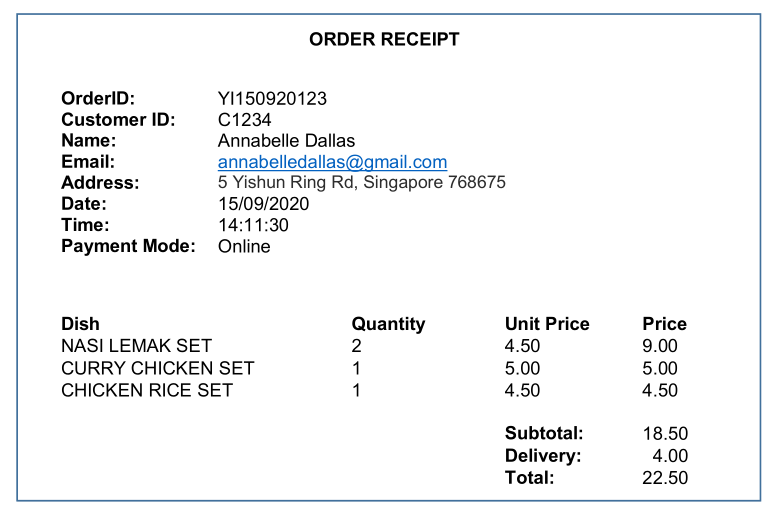
\includegraphics[width=0.5\paperwidth]{C:/Users/Admin/Desktop/Github/question_bank/LyX/static/img/9569-YIJC-2020-P1-Q5}
\par\end{center}

The restaurant assigns a unique ID to each employee and maintains
its employees\textquoteright{} information, such as their name, contact
number and bank account number. The restaurant keeps a record of the
employees\textquoteright{} delivery assignments, the date and time
when the order is successfully delivered to the customer. 
\begin{enumerate}
\item The company wants to model this application using a relational database. 
\begin{enumerate}
\item The database needs three tables to store the data for the customers\textquoteright{}
food order: \texttt{CUSTOMER}, \texttt{ORDER} and \texttt{FOOD}. 

Draw an Entity-Relationship (E-R) diagram showing the three tables
and the relationships between them. \hfill{}{[}2{]}
\item The database needs three tables to store the data for the employees\textquoteright{}
delivery assignment: \texttt{EMPLOYEE}, \texttt{ORDER} and \texttt{ASSIGNMENT}. 

Draw an Entity-Relationship (E-R) diagram showing the three tables
and the relationships between them. \hfill{}{[}2{]}
\item Draw the overall Entity-Relationship (E-R) diagram showing the five
tables and the relationships between them. \hfill{}{[}1{]}
\end{enumerate}
\item A table description can be expressed as: 

\texttt{TableName (}\texttt{\uline{Attribute1}}\texttt{, Attribute2{*},
Attribute3,...)} 

The primary key is indicated by underlining one or more attributes. 

Foreign keys are indicated using an asterisk or dashed underline. 

Write table descriptions for the five tables.\hfill{} {[}6{]}
\item Describe a method to protect data from loss or corruption.\hfill{}
{[}2{]}
\item Explain how Singapore\textquoteright s Personal Data Protection Act
(PDPA) protects the personal data of the customers and employees stored
in the database. \hfill{}{[}2{]}
\item Describe the impact of such food delivery applications on the society
and economy.\hfill{} {[}4{]}
\item With an increase in demand for food delivery, the restaurant wishes
to enhance the food delivery services to cater to the larger volume
of orders and to include more features in the application such as
real time location tracking of the food order and customers\textquoteright{}
review of the dishes, yet ensuring that the application maintains
fast performance. The restaurant is now considering using a NoSQL
DBMS instead of a relational database. 

State and explain \textbf{two} reasons why NoSQL DBMS may be more
suitable for the proposed scenario.\hfill{} {[}4{]}
\end{enumerate}
{[}SPLIT\_HERE{]}
\item \textbf{{[}YIJC/PRELIM/9569/2020/P1/Q6{]} }

A Web Developer is designing an online Sales portal for a company.
The customer needs to submit an online form to register before ordering
through the portal. 
\begin{center}
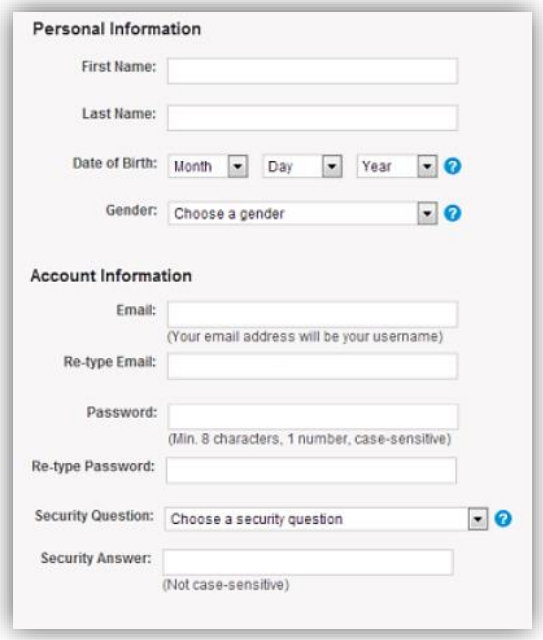
\includegraphics[width=0.25\paperwidth]{C:/Users/Admin/Desktop/Github/question_bank/LyX/static/img/9569-YIJC-2020-P1-Q6}
\par\end{center}
\begin{enumerate}
\item Explain the difference between data validation and data verification.
\hfill{}{[}2{]}
\item Describe two validation checks that the above form should perform
for the customer's inputs.\hfill{} {[}2{]}
\item Describe, with a specific example, how the customer's inputs are being
verified. \hfill{}{[}2{]}
\end{enumerate}
The web developer intends to use CAPTCHA for the above form 
\begin{center}
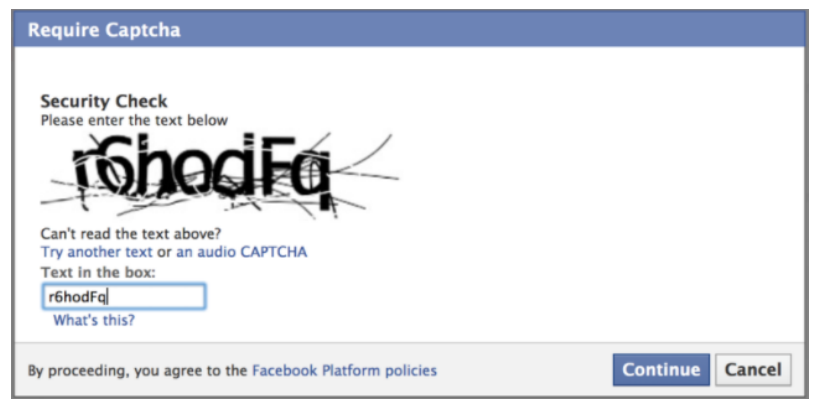
\includegraphics[width=0.3\paperwidth]{C:/Users/Admin/Desktop/Github/question_bank/LyX/static/img/9569-YIJC-2020-P1-Q6-2}
\par\end{center}
\begin{enumerate}
\item Explain what this added feature helps to verify. \hfill{}{[}2{]}
\item Describe the required server scripting to process the customer's input
on his email address and password. \hfill{}{[}4{]}
\item Describe the differences between a web application and a native application.
Explain how the developer should decide between designing a web or
a native application.\hfill{} {[}4{]}
\end{enumerate}
{[}SPLIT\_HERE{]}
\item \textbf{{[}YIJC/PRELIM/9569/2020/P1/Q7{]} }

The College\textquoteright s local area network (LAN) is connected
to the MOE Headquarter\textquoteright s LAN over the internet. 
\begin{center}
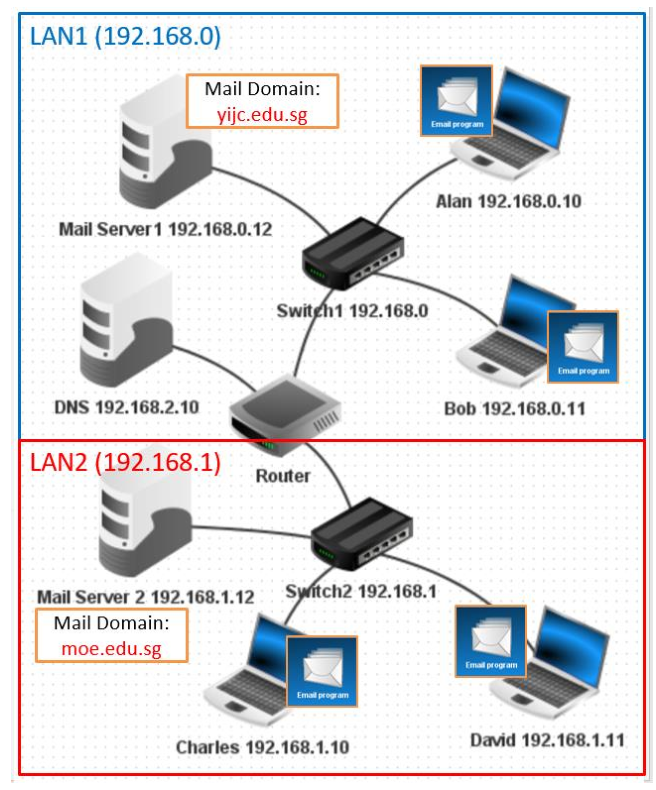
\includegraphics[width=0.5\paperwidth]{C:/Users/Admin/Desktop/Github/question_bank/LyX/static/img/9569-YIJC-2020-P1-Q7}
\par\end{center}

A staff in the college, Alan, sends an email to Charles who works
in the MOE Headquarter.
\begin{enumerate}
\item The following questions should take reference from the above network
diagram. 
\begin{enumerate}
\item Describe the function of the Domain Name System (DNS) server.\hfill{}
{[}1{]}
\item Explain how the router identifies that the MOE's Mail server is residing
in another network.\hfill{} {[}1{]}
\item Describe in detail how Alan's email is delivered and kept in the MOE's
Mail server.\hfill{} {[}2{]}
\item Describe how Charles eventually receive Alan\textquoteright s email.\hfill{}
{[}2{]}
\end{enumerate}
\item Charles forwards Alan\textquoteright s email to his colleague, David.
Describe how David could receive the email even when he is away from
the office. \hfill{}{[}2{]}
\end{enumerate}
{[}SPLIT\_HERE{]}
\item \textbf{{[}YIJC/PRELIM/9569/2020/P2/Q1{]} }

In a Battleship game, a player fires missiles within a region measuring
6 metres by 6 metres, represented with full-stops (\textquotedbl .\textquotedbl ),
to sink the ships. Each ship is represented by \textquotedbl\texttt{XXX}\textquotedbl .
The region is represented on the screen by a rectangular grid. Each
square metre of the region is represented by an x-coordinate and a
y-coordinate. The top left square metre of the region display has
\texttt{x = 0} and \texttt{y = 0}. 

\subsubsection*{Task 1.1}

In one of the games, three ships were positioned in the region as
given in the text file \texttt{GAME.TXT}. Write a program to read
in the data from this file, store it in a suitable data structure
and display on the screen as shown.

\noindent %
\noindent\begin{minipage}[t]{1\columnwidth}%
\texttt{. . . . . . }

\texttt{. . . . X . }

\texttt{X X X . X . }

\texttt{. . . . X . }

\texttt{. X X X . . }

\texttt{. . . . . . }%
\end{minipage}

\hfill{}{[}6{]}

\subsubsection*{Task 1.2}

During the game, the player cannot see the ships in the region.

\noindent %
\noindent\begin{minipage}[t]{1\columnwidth}%
\texttt{. . . . . . }

\texttt{. . . . . . }

\texttt{. . . . . . }

\texttt{. . . . . . }

\texttt{. . . . . . }

\texttt{. . . . . .}%
\end{minipage}

Write program code to allow the player to fire 5 missiles targeting
at specific locations, one at a time after observing each outcome.
The player will input an x-coordinate and y-coordinate for each targeted
location.

If the missile strikes any part of a ship, the damaged square metre
will be represented with an \textquotedbl\texttt{S}\textquotedbl ,
otherwise an \textquotedbl\texttt{O}\textquotedbl{} to represent
it has missed. A sunken ship will be represented by \textquotedbl\texttt{SSS}\textquotedbl .

\noindent %
\noindent\begin{minipage}[t]{1\columnwidth}%
one missile which missed the ship

\bigskip{}

\texttt{O . . . . .}

\texttt{. . . . . .}

\texttt{. . . . . .}

\texttt{. . . . . .}

\texttt{. . . . . .}

\texttt{. . . . . .}%
\end{minipage}

\noindent %
\noindent\begin{minipage}[t]{1\columnwidth}%
another missile which struck the ship

\bigskip{}

\texttt{O . . . . .}

\texttt{. . . . . .}

\texttt{. S . . . .}

\texttt{. . . . . .}

\texttt{. . . . . .}

\texttt{. . . . . .}%
\end{minipage}

The program code should also display the positions of all the ships
at the end of the game.

\noindent %
\noindent\begin{minipage}[t]{1\columnwidth}%
\texttt{O . . . . . }

\texttt{. . . . X . }

\texttt{S S S . X . }

\texttt{. . . . X . }

\texttt{. X X S . . }

\texttt{. . . . . .}%
\end{minipage}

\hfill{}{[}7{]} 

Download your program code and output for Task 1.1 and 1.2 as 

\texttt{Task1\_<your name>\_<centre number>\_<index number>.ipynb}

\subsubsection*{Task 1.3}

Write server and client program for this asymmetric Battleship game
where a server display the region and the player (the client) selects
the target locations for his missiles. After firing each missile,
the server returns an updated display for the region indicating a
strike or a miss. Once the player fires his last missile, the server
will display the positions of all the ships, together with the damages
and misses, and both the client and server quit the game. \hfill{}{[}12{]}

Download your server and client program code for Task 1.3 as

\texttt{Task1\_server\_<your name>\_<centre number>\_<index number>.py }

\texttt{Task1\_client\_<your name>\_<centre number>\_<index number>.py}

{[}SPLIT\_HERE{]}
\item \textbf{{[}YIJC/PRELIM/9569/2020/P2/Q2{]} }

The file \texttt{SONG.TXT} contains the lyrics of the song, Count
on me Singapore. The task is to read every word from the file, store
it in a suitable data structure, sort the words and perform searches
based on word and count.

\subsection*{Task 2.1}

Write program code to:
\begin{itemize}
\item read the words from the file and store them in a suitable data structure,
\item sort the words in alphabetical order using \textbf{quick sort}, 
\item write each word and their number of occurrence in a text file, WORDCOUNT.TXT,
where the next word is on a new line. {[}12{]}
\end{itemize}
A sample of the \texttt{WORDCOUNT.TXT} for the first 5 lines is as
follows:

\noindent %
\noindent\fbox{\begin{minipage}[t]{1\columnwidth - 2\fboxsep - 2\fboxrule}%
\texttt{a 5 }

\texttt{achieve 12 }

\texttt{air 1 }

\texttt{all 1 }

\texttt{and 9}%
\end{minipage}}

\subsection*{Task 2.2}

Write program code to:
\begin{itemize}
\item read the words and counts from the \texttt{WORDCOUNT.TX}T file 
\item allow the user to select the following options:

\noindent %
\noindent\begin{minipage}[t]{1\columnwidth}%
\texttt{1. Search for a word }

\texttt{2. Search for word(s) based on count}

\texttt{3. Quit program}%
\end{minipage}
\item take in user input for the word or the count 
\item if found, display the word and its count, else 
\item display \textquotedbl\texttt{Not Found}\textquotedbl{} display appropriate
error messages for invalid user input \hfill{}{[}6{]}
\end{itemize}

\subsection*{Task 2.3}

Design test data for your program written in \textbf{Task 2.2}, provide
evidence of testing that includes:
\begin{itemize}
\item search for a word that is contained in the file 
\item search for a word that is not contained in the file
\item search for word(s) with a count that is contained in the file 
\item search for word(s) with a count that is not contained in the file
\hfill{} {[}2{]}
\end{itemize}
Download your program code and output for Task 2 as 

\texttt{Task2\_<your name>\_<centre number>\_<index number>.ipynb}

{[}SPLIT\_HERE{]}
\item \textbf{{[}YIJC/PRELIM/9569/2020/P2/Q3{]} }

The task is to store words in nodes that is contained within a linked
list data structure. A node contains a word, the word category and
a next pointer. The pointers link the word items in proper grammatical
order based on their word category (\textquoteleft N\textquoteright :
noun, \textquoteleft V\textquoteright : verb, \textquoteleft D\textquoteright :
determiner, \textquoteleft J\textquoteright : adjective). The unused
nodes are linked as shown below. The first unused node is the position
where the new word item is to be stored.
\begin{center}
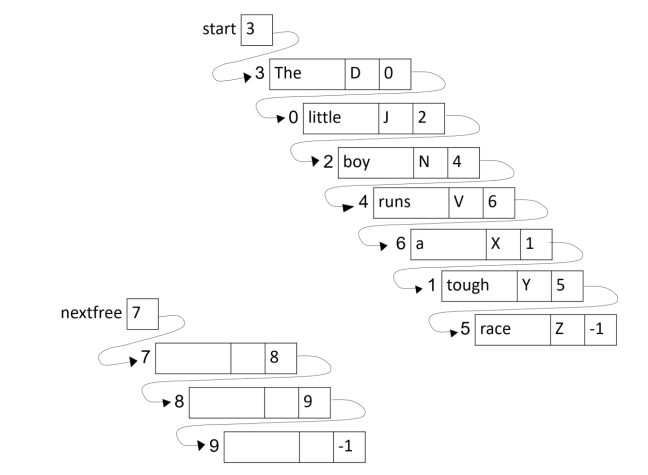
\includegraphics[width=0.5\paperwidth]{C:/Users/Admin/Desktop/Github/question_bank/LyX/static/img/9569-YIJC-2020-P2-Q3-1}
\par\end{center}

The diagram shows the linked list with:
\begin{itemize}
\item the words and their respective category inserted in the following
order: 
\begin{itemize}
\item \texttt{'little', 'J' }
\item \texttt{'tough', 'J' }
\item \texttt{'boy', 'N' }
\item \texttt{'The', 'D' }
\item \texttt{'runs', 'V' }
\item \texttt{'race', 'N' }
\item \texttt{'a', 'D'}
\end{itemize}
\item the unused nodes linked together
\end{itemize}
Each node is implemented as an instance of the class Node. The class
Node has the following UML class diagram:
\begin{center}
\begin{tabular}{|l|}
\hline 
\hspace{0.25\columnwidth}Node\tabularnewline
\hline 
\texttt{word: STRING}\tabularnewline
\texttt{category: STRING}\tabularnewline
\texttt{next: INTEGER}\tabularnewline
\hline 
\texttt{constructor()}\tabularnewline
\texttt{set\_word(w: STRING)}\tabularnewline
\texttt{set\_category(c: STRING)}\tabularnewline
\texttt{set\_next(n: INTEGER)}\tabularnewline
\texttt{get\_word(): STRING}\tabularnewline
\texttt{get\_category(): STRING}\tabularnewline
\texttt{get\_next(): INTEGER}\tabularnewline
\hline 
\end{tabular}
\par\end{center}

The \texttt{LinkedList} class is implemented as follows: 
\begin{itemize}
\item Attributes
\begin{itemize}
\item \texttt{sentence : ARRAY{[}0:9{]} of Node -} The linked list data
structure that contains 10 nodes.
\item \texttt{start : INTEGER} - Index for the start position of the linked
list. 
\item \texttt{nextfree : INTEGER} - Index for the next unused node.
\end{itemize}
\item Methods
\begin{itemize}
\item \texttt{\_\_init\_\_ : PROCEDURE} - Sets all the node data values
to \textquoteleft empty string\textquoteright . Set pointers to indicate
all nodes are unused and linked. Initialise values for start and nextfree.
\item \texttt{isempty : FUNCTION RETURNS BOOLEAN} - Tests for empty linked
list.
\item \texttt{isfull : FUNCTION RETURNS BOOLEAN} - Tests for no unused nodes.
\item \texttt{display : PROCEDURE} - Displays the contents of sentence in
index order. 
\item \texttt{insert : PROCEDURE} - Adds a new word and its category to
the linked list. 
\item \texttt{traversal : PROCEDURE} - Displays the simple sentence obtained
from the linked list.
\end{itemize}
\end{itemize}
The index of the first available node is indicated by \texttt{nextfree}.
The initial values of \texttt{start} and \texttt{nextfree} is -1 and
0 respectively.

\subsection*{Task 3.1}

Write the program code to define the \texttt{Node} and \texttt{LinkedList}
classes. 

Do not attempt to write the methods \texttt{insert} and \texttt{traversal}
at this stage. \hfill{} {[}10{]}

\subsection*{Task 3.2}

Write program code to create a LinkedList object and run the display
method to confirm the initial values of the pointers, word and category
values when the linked list is empty. \hfill{}{[}2{]}

A simple sentence contains words from different category arranged
in the manner as illustrated: 

(\textquoteleft N\textquoteright : noun, \textquoteleft V\textquoteright :
verb, \textquoteleft D\textquoteright : determiner, \textquoteleft J\textquoteright :
adjective)

Verb come between two nouns.

Determiner comes before a noun, adjective comes before a noun and
after a determiner.
\noindent \begin{center}
\begin{tabular}{|c|c|c|}
\hline 
boy & runs & race\tabularnewline
\hline 
N & V & N\tabularnewline
\hline 
\end{tabular}
\par\end{center}

\noindent \begin{center}
\begin{tabular}{|c|c|c|c|c|}
\hline 
The & boy  & runs & a & race\tabularnewline
\hline 
D & N & V & D & N\tabularnewline
\hline 
\end{tabular}
\par\end{center}

\noindent \begin{center}
\begin{tabular}{|c|c|c|c|c|c|c|}
\hline 
The & little & boy & runs & a & tough & race\tabularnewline
\hline 
D & J & N & V & D & J & N\tabularnewline
\hline 
\end{tabular}
\par\end{center}

In order to aid the process of inserting the words in their correct
position in the linked list, the code letter \textquoteleft X\textquoteright ,
\textquoteleft Y\textquoteright{} and \textquoteleft Z\textquoteright{}
is used in place of the second set of \textquoteleft D\textquoteright ,
\textquoteleft J\textquoteright , \textquoteleft N\textquoteright{}
respectively, so that the correct position can be determined by comparing
the category when traversing down the linked list.
\noindent \begin{center}
\begin{tabular}{|c|c|c|c|c|c|c|}
\hline 
The & little & boy & runs & a & tough & race\tabularnewline
\hline 
D & J & N & V & X & Y & Z\tabularnewline
\hline 
\end{tabular}
\par\end{center}

The following pseudocode (available in PSEUDOCODE\_TASK\_3\_3.TXT
) can be used to add a word and its category to the linked list.

\noindent %
\noindent\begin{minipage}[t]{1\columnwidth}%
\texttt{PROCEDURE insert(new\_word, new\_category)}

\texttt{\bigskip{}
}

\texttt{\qquad{}//check if Linked List is full }

\texttt{\qquad{}IF nextfree = -1 THEN }

\texttt{\qquad{}\qquad{}RETURN 'Linked List is Full' }

\texttt{\qquad{}ENDIF }

\texttt{\bigskip{}
}

\texttt{\qquad{}//linked list is not full, safe to insert new word }

\texttt{\qquad{}sentence{[}nextfree{]}.word <- new\_word }

\texttt{\qquad{}sentence{[}nextfree{]}.category <- new\_category}

\texttt{\bigskip{}
}

\texttt{\qquad{}IF start = -1 THEN //inserting into empty list }

\texttt{\qquad{}\qquad{}start <- nextfree}

\texttt{\qquad{}\qquad{}temp <- sentence{[}start{]}.next }

\texttt{\qquad{}\qquad{}sentence{[}start{]}.next <- -1 }

\texttt{\qquad{}\qquad{}nextfree <- temp}

\texttt{\bigskip{}
}

\texttt{\qquad{}ELSE }

\texttt{\qquad{}// traverse down the linked list to search for position
to}

\texttt{\qquad{}// insert }

\texttt{\qquad{}\qquad{}current <- start //pointer of current node }

\texttt{\qquad{}\qquad{}previous <- -1 //pointer of previous node }

\texttt{\qquad{}\qquad{}inserted <- FALSE //flag to check for insertion}

\texttt{\bigskip{}
}

\texttt{\qquad{}\qquad{}WHILE current > -1 AND inserted = FALSE}

\texttt{\qquad{}\qquad{}\qquad{}IF sentence{[}current{]}.category
> new\_category THEN \bigskip{}
}

\texttt{\qquad{}\qquad{}\qquad{}//position found, insert before
current node }

\texttt{\qquad{}\qquad{}\qquad{}\qquad{}IF current = start THEN }

\texttt{\qquad{}\qquad{}\qquad{}\qquad{}\qquad{}//check if current
equals to start}

\texttt{\qquad{}\qquad{}\qquad{}\qquad{}\qquad{}start <- nextfree }

\texttt{\qquad{}\qquad{}\qquad{}\qquad{}ELSE }

\texttt{\qquad{}\qquad{}\qquad{}\qquad{}\qquad{}sentence{[}previous{]}.next
<- nextfree}

\texttt{\qquad{}\qquad{}\qquad{}\qquad{}ENDIF \bigskip{}
}

\texttt{\qquad{}\qquad{}\qquad{}\qquad{}temp <- sentence{[}nextfree{]}.next}

\texttt{\qquad{}\qquad{}\qquad{}\qquad{}sentence{[}nextfree{]}.next
<- current}

\texttt{\qquad{}\qquad{}\qquad{}\qquad{}nextfree <- temp}

\texttt{\qquad{}\qquad{}\qquad{}\qquad{}inserted <- TRUE}

\texttt{\bigskip{}
}

\texttt{\qquad{}\qquad{}\qquad{}ELIF sentence{[}current{]}.category
< new\_category THEN }

\texttt{\qquad{}\qquad{}\qquad{}\qquad{}previous <- current }

\texttt{\qquad{}\qquad{}\qquad{}\qquad{}current <- sentence{[}current{]}.next }

\texttt{\bigskip{}
}

\texttt{\qquad{}\qquad{}\qquad{}ELSE THEN }

\texttt{\qquad{}\qquad{}\qquad{}\qquad{}IF new\_category = 'N'
THEN }

\texttt{\qquad{}\qquad{}\qquad{}\qquad{}\qquad{}new\_category
<- 'Z'}

\texttt{\qquad{}\qquad{}\qquad{}\qquad{}ENDIF }

\texttt{\qquad{}\qquad{}\qquad{}\qquad{}IF new\_category = 'D'
THEN }

\texttt{\qquad{}\qquad{}\qquad{}\qquad{}\qquad{}new\_category
<- 'X' }

\texttt{\qquad{}\qquad{}\qquad{}\qquad{}ENDIF }

\texttt{\qquad{}\qquad{}\qquad{}\qquad{}IF new\_category = 'J'
THEN }

\texttt{\qquad{}\qquad{}\qquad{}\qquad{}\qquad{}new\_category
<- 'Y' }

\texttt{\qquad{}\qquad{}\qquad{}\qquad{}ENDIF }

\texttt{\bigskip{}
}

\texttt{\qquad{}\qquad{}\qquad{}\qquad{}previous <- current }

\texttt{\qquad{}\qquad{}\qquad{}\qquad{}current <- sentence{[}current{]}.next}

\texttt{\qquad{}\qquad{}\qquad{}\qquad{}sentence{[}nextfree{]}.category
<- new\_category}

\texttt{\qquad{}\qquad{}\qquad{}ENDIF}

\texttt{\qquad{}\qquad{}ENDWHILE}

\texttt{\bigskip{}
}

\texttt{\qquad{}\qquad{}IF inserted = False THEN }

\texttt{\qquad{}\qquad{}\qquad{}sentence{[}previous{]}.next <-
nextfree }

\texttt{\qquad{}\qquad{}\qquad{}temp <- sentence{[}nextfree{]}.next }

\texttt{\qquad{}\qquad{}\qquad{}sentence{[}nextfree{]}.next <-
-1 }

\texttt{\qquad{}\qquad{}\qquad{}nextfree <- temp }

\texttt{\qquad{}\qquad{}ENDIF }

\texttt{\bigskip{}
}

\texttt{\qquad{}ENDIF}

\texttt{ENDPROCEDURE}%
\end{minipage}

\subsection*{Task 3.3}

Write code to implement \texttt{insert} method from this pseudocode.
You may use the text file \texttt{PSEUDOCODE\_TASK\_3\_3.TXT} as a
basis for writing your code. \hfill{}{[}8{]}

\subsection*{Task 3.4:}

Write code to insert the following into the linked list created in
\textbf{Task 3.2} and display its contents:
\begin{itemize}
\item 'little', 'J' 
\item 'tough', 'J' 
\item 'boy', 'N' 
\item 'The', 'D' 
\item 'runs', 'V' 
\item 'race', 'N' 
\item 'a', 'D' \hfill{}{[}2{]}
\end{itemize}

\subsection*{Task 3.5:}

Write code to implement traversal method which displays the simple
sentence obtained from traversing the linked list and run it. 

The expected output should look like this:
\noindent \begin{center}
\texttt{The little boy runs a tough race. }\hfill{}{[}8{]}
\par\end{center}

Download your program code and output for Task 3 as

\texttt{Task3\_<your name>\_<centre number>\_<index number>.ipynb}

{[}SPLIT\_HERE{]}
\item \textbf{{[}YIJC/PRELIM/9569/2020/P2/Q4{]} }

\emph{SafeEnter} is a digital check-in system that tracks the people
visiting the public places, to prevent and control the transmission
of COVID-19 through contact tracing.
\begin{center}

\includegraphics[width=0.25\paperwidth]{C:/Users/Admin/Desktop/Github/question_bank/LyX/static/img/9569-YIJC-2020-P2-Q4-1}
\par\end{center}

\subsection*{Task 4.1}

Create a HTML file called \texttt{index.html} to display the Check-In
form for people to input their particulars and other details. (Use
the picture \texttt{IN.JPG} provided.) {[}5{]}
\begin{center}
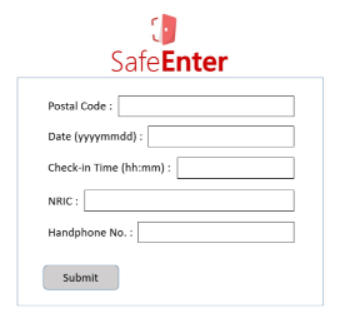
\includegraphics[width=0.25\paperwidth]{C:/Users/Admin/Desktop/Github/question_bank/LyX/static/img/9569-YIJC-2020-P2-Q4-2}
\par\end{center}

\noindent \begin{center}
Check-In Form
\par\end{center}

\subsection*{Task 4.2}

Write program code, \texttt{server.py}, for the back-end server to
display the Check-In form on the clients\textquoteright{} browser
when they scan a QR-code which links to the SafeEnter website. The
server script should include a route \textquoteleft \texttt{/checkin}\textquoteright{}
to receive the inputs from the client, the program code should: 
\begin{itemize}
\item prevent the user from accessing the \textquoteleft \texttt{/checkin}\textquoteright{}
route directly 
\item receive all the inputs in the Check-In form
\item reject empty or null inputs
\item append the new entry into the \texttt{event} table in the given database
\texttt{covid.db }
\item reply by sending a \texttt{checkout.html} page back to the client\textquoteright s
browser, displaying the following Check-Out form, which is to be used
when leaving the venue (Use the picture \texttt{OUT.JPG} provided.)\texttt{
}\hfill{}{[}12{]}
\end{itemize}
\begin{center}
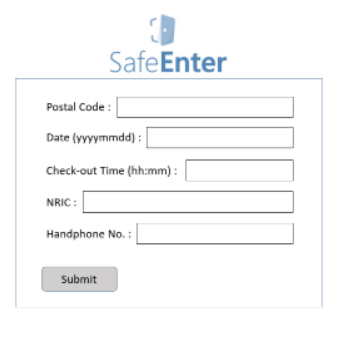
\includegraphics[width=0.25\paperwidth]{C:/Users/Admin/Desktop/Github/question_bank/LyX/static/img/9569-YIJC-2020-P2-Q4-3}
\par\end{center}

\noindent \begin{center}
Check-Out Form
\par\end{center}

\subsection*{Task 4.3}

Modify the program code, \texttt{server.py}, and include an additional
route \textquoteleft \texttt{/checkout}\textquoteright{} to receive
the inputs from the client\textquoteright s Check-Out form when they
leave the venue. The program code should: 
\begin{itemize}
\item allow the user from accessing the \textquoteleft /checkout\textquoteright{}
route directly 
\item receive all the inputs in the Check-Out form 
\item reject empty or null inputs 
\item update the corresponding entry in the \texttt{event} table in the
\textbf{given} database \texttt{covid.db }\hfill{}{[}8{]}
\end{itemize}
Download the files for your program codes for Task 4 as 

\texttt{Task4\_<your name>\_<centre number>\_<index number>\_index.html }

\texttt{Task4\_<your name>\_<centre number>\_<index number>\_checkout.html}

\texttt{Task4\_<your name>\_<centre number>\_<index number>\_server.py }

\texttt{Task4\_<your name>\_<centre number>\_<index number>\_covid.db}

{[}SPLIT\_HERE{]}
\end{enumerate}

\end{document}
